% % % % % % % % % % % % % % % % % % % % % %
% Präambel
% % % % % % % % % % % % % % % % % % % % % %

\documentclass[paper = a4, fontsize = 12pt, parskip = half]{scrartcl} % Doku: "scrguide"
\usepackage[ngerman]{babel} % Sprachenunterstützung für LaTeX; Doku: "gerdoc"7
\usepackage[T1]{fontenc} % Schriftkodierung
\usepackage[utf8]{inputenc} % Eingabekodierung
\usepackage{lmodern} % Schrift: Latin Modern

\usepackage{scrlayer-scrpage}
\usepackage{microtype} % mikrotypographische Erweiterungen von pdfTeX; s.a. microtype-DE
\usepackage{amsmath} % AMSmath-Paket der American Mathematical Society (AMS)
\usepackage{eurosym} % das Euro-Zeichen (?) z.B. mit \EUR{}
\usepackage{grffile} % erweiterte Unterstützung für Grafikdateinamen (z.B. mehrere Punkte)
\usepackage{graphicx} % Einbinden von Grafiken; Doku: "grfguide"
\usepackage{url} % Querverweise können im Text hervorgehoben werden
\usepackage{hyperref} % Querverweise in Hyperlinks umwandeln
\usepackage{setspace} % Ermöglicht Änderungen des Zeilenabstands
\usepackage{paralist} % Erweiterung der Listenumgebungen\usepackage{hyperref}
\usepackage{csquotes} % advanced facilities for inline and display quotations
\usepackage{wrapfig} % Grafiken mit Text umfließen
\usepackage{color}

\usepackage[style=ieee]{biblatex}
\addbibresource{library.bib}

\hypersetup{pdfborder={0 0 0}}
\setkomafont{captionlabel}{\small\sffamily\bfseries}
\addtokomafont{caption}{\small}

%% set heading and footer
%% scrheadings default: 
%% footer - middle: page number
\pagestyle{scrheadings}
%%\automark[subsection]{section}
%% user specific
%% usage:
%% \position[heading/footer for the titlepage]{heading/footer for the rest of the document}
%% heading - left
% \ihead[]{}
%% heading - center
% \chead[]{}
%% heading - right
% \ohead[]{}
%% footer - left
% \ifoot[]{}
%% footer - center
% \cfoot[]{}
%% footer - right
% \ofoot[]{}

% % % % % % % % % % % % % % % % % % % % % %

\begin{document}
% % % % % % % % % % % % % % % % % % % % % %
% Beginn der Titelseite 
% % % % % % % % % % % % % % % % % % % % % %

\begin{titlepage}

    \begin{center}
        
\includegraphics[width=8cm]{images/logo_aau.png} \\
        \vspace{8mm}
        \huge\textbf{Alpen-Adria-Universität Klagenfurt} \\
        \vspace{3mm}
        Fakultät für Technische Wissenschaften \\
        \vspace{3mm}
        Institut für Informationstechnologie (ITEC)\\
        \vspace{3mm}
    \end{center}
    
    \vspace{5mm}
    
    \begin{center}
        \textbf{Lehrveranstaltung: \\
            Seminar aus Angewandte Informatik} \\
        \vspace{2mm}
        LV-Leiter: Univ.-Prof. Dipl.-Ing. Dr. Hermann Hellwagner \\
        LV-Nr.: 622.000 \\
        SS 2021
    \end{center}
    
    \vspace{15mm}
    
    \begin{center}
        \Large\textbf{MPEG-DASH Standard} \\
        \vspace{2mm}
        \normalsize Dynamic Adaptive Streaming over HTTP
    \end{center}
    
    \vspace{40mm}
    
    \begin{flushleft}
        \textbf{Andreas Kogler} \\
        E-Mail: andrkogler@edu.aau.at \\
        Studienrichtung: Bachelorstudium Angewandte Informatik \\
        Matrikel-Nr.: 11702050\\
        Datum: \today
    \end{flushleft}
    
\end{titlepage}

% % % % % % % % % % % % % % % % % % % % % %

% % % % % % % % % % % % % % % % % % % % % % 
% Inhalts- und Abbildungsverzeichnis
% % % % % % % % % % % % % % % % % % % % % %

% \thispagestyle{empty}
% \tableofcontents
% \listoffigures
% \listoftables

% % % % % % % % % % % % % % % % % % % % % %

% % % % % % % % % % % % % % % % % % % % % % 
% Beginn des Dokuments
% % % % % % % % % % % % % % % % % % % % % %

% \newpage
\setcounter{page}{1}
\onehalfspacing

\section*{Abstract}
Wie der jährlich herausgegebene Cisco Visual Networking Index \cite{cisco_syst_inc_cisco_2017} zeigt, steigt der Anteil von Videodaten im Internet rapide. Mit Ende 2021 sollen Videodaten 80\% des globalen Gesamtdatenvolumens ausmachen \cite{cisco_syst_inc_cisco_2017}.

Das vormals verbreitete \textit{Real-Time Transport Protocol} operiert unter der Annahme eines \textit{managed} IP-Netzwerks, wohingegen in modernen Umgebungen Content Distribution Networks (CDNs) verwendet werden \cite{sodagar_mpeg-dash_2011}. Während in managed IP-Netzwerken Server für die Verteilung der (Video-)Daten fest vorgegeben sind, können sich Server in CDNs dynamisch aufgrund einer Reihe von Kennzahlen regelmäßig ändern \cite{buyya_content_2008}. Um diesem Problem und der Vielfalt an proprietären Streamingstandards zu entgegnen, hat MPEG einen Standard für \textit{Dynamic Adaptive Streaming over HTTP}, auch bekannt als MPEG-DASH, entwickelt \cite{sodagar_mpeg-dash_2011}.

Im Mittelpunkt steht dabei die dynamische Bitratenadaptierung der Videodaten je nach verfügbarer Bandbreite von Netzwerk und Endgerät. Da sich die verfügbare Bandbreite während der Wiedergabe des Videos ändern kann, müssen verschiedene Algorithmen zur dynamischen Selektion der Bitrate angewandt werden \cite{bentaleb_survey_2019}.

Die eigentlichen Audio- und Video-Bitströme werden dabei in kleinere Segmente unterteilt welche wiederum in verschiedenen Qualitätsstufen für den Client zur Auswahl stehen. Jedes Segment besitzt eine eindeutige URL, über die es mittels HTTP GET-Request angefragt werden kann. Alle verfügbaren Segment-URLs werden in der \textit{Multimedia Presentation Description (MPD)} angegeben. Durch Einlesen dieser XML-Datei am Anfang des Streamingprozesses lernt der Client über alle verfügbaren Qualitätsstufen und kann diese gemäß des verwendeten Algorithmus auswählen \cite{sodagar_mpeg-dash_2011}.

MPEG-DASH definiert in seiner Spezifikation lediglich die Segmentformate, den Aufbau der MPD-Datei und die verpflichtende Verwendung von HTTP/1.1 \cite{mpeg_dynamic_2013}. Viele weitere Aspekte wie beispielsweise Austausch der MPD, Codierung der Daten oder Verhalten bei der Bitratenadaption sind Gegenstand der jeweiligen Implementierung \cite{sodagar_mpeg-dash_2011}.

Diese Arbeit bietet einen Überblick zu MPEG-DASH allgemein, legt ihren Schwerpunkt jedoch auf durch den Standard vorgegebene Aspekte. 
Nicht-standardisierte Teile werden konzeptuell eingeführt und anhand aktueller Lösungsbeispiele konkretisiert. Für Details wird an den jeweiligen Stellen auf tiefergehende Lektüre verwiesen.

\section{Warum Adaptives Streaming?}
Die Anzahl potentieller Endgeräte mit denen Menschen Videostreams konsumieren hat sich in den letzten Jahren stark erhöht. Neben klassischen Medien wie PC und TV-Receiver haben sich vorallem Smartphones, Tablets und Spielkonsolen im täglichen Gebrauch der NutzerInnen etabliert.

Diese Endgeräte weisen unterschiedliche Charakteristiken auf, welche die Anforderungen an das Videoformat und dessen Übertragung stark beeinflussen. Vorrangig betrachten wir im Kontext von Videostreaming die Bildschirmgröße und Auflösung sowie die Verfügbare Bandbreite des Endgeräts und des Netzwerks.
Es reicht also nicht ein Video in einer einzigen Version Serverseitig zu speichern. Während die Qualität für einen Full-HD Computerbildschirm völlig ausreichend sein könnte, würde sie auf einem 4k-TV aufgrund zu geringer Auflösung verschwomme angezeigt werden und wäre für einen Smartphone-Bildschirm unnötig groß. Letzteres lässt anmuten dass auch das Netzwerk eine zentrale Rolle im Videostreaming spielt.

Smartphones, die mit steigender Tendenz einen Großteil des globalen Internettraffics ausmachen, sind zu einem Großteil über das Mobilfunknetz an das Internet angebunden. Hier kann es insbesondere zu Schwankungen in der verfügbaren Bandbreite am Endgerät und im Netzwerk kommen. Ein Einbruch der verfügbaren Bandbreite führt zu Pufferwartezeiten bei der Wiedergabe, was die QoE (Quality of Experience) wiederum stark negativ beeinflusst. 

Dieser Umstand führte schließlich zur Idee des adaptiven Videostreamings. Ein Konzept in dem die Bitrate des zu übertragenden Videos während der Wiedergabe dynamisch an die Netzwerkgegebenheiten angepasst (adaptiert) wird. Das führt bei Netzwerkengpässen zwar dazu dass Teile des konsumierten Videos mit geringerer Qualität wiedergegeben werden, vermeidet allerdings gefürchtete Pufferwartezeiten und beeinträchtigt die QoE für den Benutzer nur marginal.

\section{Adaptive-Streaming Standards - Überblick}
Adaptives Streaming ist grundsätzlich ein generelles Konzept und keine konkrete Technologie. Zur konkreten Umsetzung haben sich in den letzten Jahren zwei große Standards gebildet. Einerseits wurde von Apple das proprietäre Protokoll HLS (HTTP Live Streaming) entwickelt, während die Moving Pictures Expert Group (MPEG) den offenen Standard MPEG-DASH (Dynamic Adaptive Streaming over HTTP) entwickelt hat. Der DASH-Standard wurde 2012 offiziell von MPEG unter der ISO/IEC-Nummer 23009 veröffentlicht und besteht aus acht Parts:

\begin{itemize}
    \item \textbf{Part 1:} Media presentation description and segment formats
    \item \textbf{Part 2:} Reference software and conformance
    \item \textbf{Part 3:} Implementation guidelines
    \item \textbf{Part 4:} Format Independent Segment encryption and authentication
    \item \textbf{Part 5:} Server and network assisted DASH (SAND)
    \item \textbf{Part 6:} DASH with Server Push and WebSockets
    \item \textbf{Part 7:} Delivery of CMAF content with DASH
    \item \textbf{Part 8:} Session based DASH operation
\end{itemize}

HLS wurde 2009 von Apple veröffentlicht.

Beide Technologien setzen für die Übertragung auf der Applikationsebene das Hyper Text Transfer Protocol (HTTP) ein. Beide Protokolle werden von einer weiten Palette an Endgeräten unterstützt. Ausnahme ist die Unterstützung bei Apple Geräten. Der Safari-Browser, welcher bei iPhone, iPad, Mac und AppleTV als Standard ausgeliefert wird, unterstützt nativ kein MPEG-DASH sondern nur den hauseigenen HLS-Standard.

\section{Einführung in MPEG-DASH}
Um adaptives Streaming via MPEG-DASH zu ermöglichen wird die Mediendatei zunächst in mehrere, kleine Segmente zwischen zwei und zehn Sekunden Länge aufgeteilt. Jedes dieser Segmente wird anschließend in verschiedenen Qualitätsstufen kodiert. Segmente in einer höheren Qualitätsstufe benötigen mehr Speicherplatz und später auch mehr Bandbreite bei der Übertragung. Die so entstandenen Segmente werden schließlich auf einen Webserver hochgeladen, wo sie mittels HTTP GET-Requests angefragt werden können. 

Clientseitig übernimmt DASH-konforme Software die Kommunikation mit dem Webserver. Um dem Client einen Überblick über die verfügbaren Qualitätsstufen des angefragten Videos zu bieten wird vom Server zu Beginn die \textit{Media Presentation Description}, kurz \textit{MPD}, bereitgestellt. Ein Teil der Clientsoftware misst permanent die zur Verfügung stehende Bandbreite und bestimmt so in welcher Qualitätsstufe ein Segment angefragt wird. Dieser Teil der Software wird \textit{Bitrate Adaption Algorithm} genannt. 

\begin{center}
    \begin{figure}
        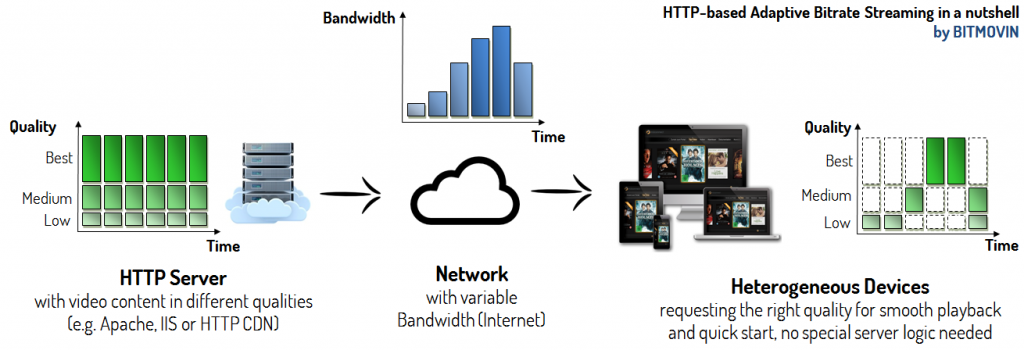
\includegraphics[width=14cm]{images/adaptive-streaming-basic.png}
        \caption{https://bitmovin.com/dynamic-adaptive-streaming-http-mpeg-dash/}
    \end{figure}
\end{center}


\subsection{HTTP (grundsätzlich, warum für Streaming geeignet?)}
DASH schreibt die Nutzung von HTTP/1.1 oder 1.0 im Streamingprozess vor. Das ist vorallem auf eine Auswahl an Features zurückzuführen, die in früheren HTTP-Versionen nicht vorhanden ist. Erkläre basic GET-Requests, welche Features mit HTTP 1.0 nicht genutzt werden usw.

\subsection{Media Presentation Description (MPD)}
Bevor der Streamingprozess beginnt muss die MPD zwischen Client und Server ausgetauscht werden. Der Austauschprozess wird dabei nicht vom Standard vorgegeben sondern ist von der Implementierung des jeweiligen Anbieters abhängig.

Eine MPD-Datei dient als \textit{Inhaltsverzeichnis} für den Client, bietet einen Überblick über sämtliche vorhandene Mediendaten (Video, Audio, Untertitel), deren Eigenschaften und die zugehörige URL an die HTTP-Requests gestellt werden um das jeweilige Segment zu erhalten.

Die Dateistruktur wird strikt durch den Standard vorgegeben. MPD-Dateien folgen einem durch den Standard vorgegebenen XML-Schema. Folgende Grafik veranschaulicht die wichtigsten Komponenten einer MPD auf die in den kommenden Kapiteln näher eingegangen wird:

\begin{center}
    \begin{figure}[h!]
        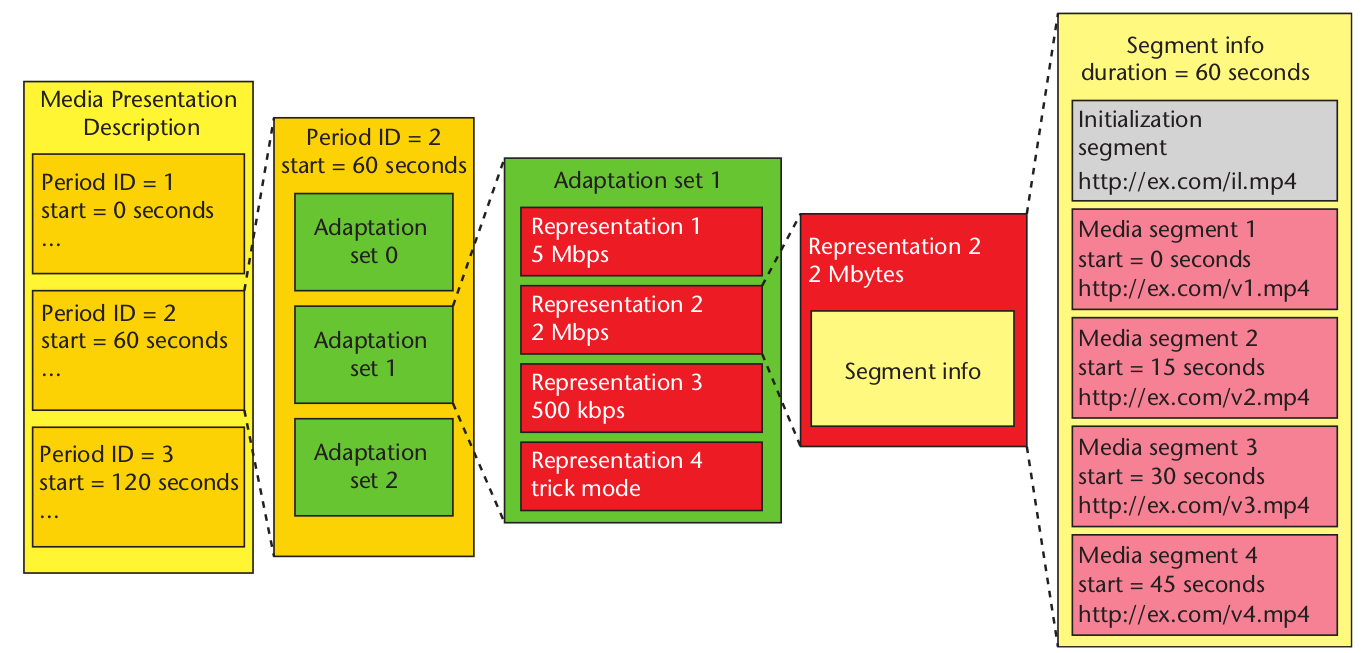
\includegraphics[width=12cm]{images/mpd-structure.png}
        % https://www.bogotobogo.com/VideoStreaming/images/mpeg_dash/MPEG-DASH-Tutorial.pdf
        \caption{Quelle siehe Kommentar}
    \end{figure}
\end{center}

\textbf{Notiz:} Es werden pro Abschnitt nur Attribute und Sub-Elemente besprochen die laut ISO/IEC 23009-1 als \textit{Mandatory}, also unbedingt notwendig, gekennzeichnet sind oder dem Zweck eines anschaulichen Beispiels dienen. Für eine vollständige Übersicht wird auf den offiziellen Standard ISO/IEC 23009 Part 1 (Media Presentation Description and Segment formats) verwiesen.

\subsubsection{XML-Schema}

\subsubsection{Root-Element <MPD>}
Jede MPD besitzt genau ein einziges <MPD>-Tag als Root-Element welches auf die XML-Deklaration in der ersten Zeile und der Einbindung des Schemas / Angabe des Namespaces folgt. 
Folgende Attribute sind für ein valides MPD-Tag zwingend notwendig:

\begin{itemize}
    \item \textbf{profiles}: Listet die unterstützten Medienprofile auf. Eine Übersicht über verfügbare Profile sowie deren Notation werden in Abschnitt \ref{profiles} behandelt.
    \item \textbf{minBufferTime}: Minimiale Zeitdauer an Segmenten die ein Client im Puffer bereithalten muss um Playback starten zu können. Angabe als ISO 8601-Duration. Details zum Format im Abschnitt \ref{iso8601_duration}.
\end{itemize}

Direkt unter dem Root-Tag können außerdem BaseURL-Elemente spezifiziert werden. Eine BaseURL kann alternative URLs für Mediendaten liefern.
Die Basis-URL wird gemäß IETF RFC3986 (5.1.1 - 5.1.4) eruiert. Wird mit folgenden Schritten versucht eine Basis-URL zu finden:

\begin{enumerate}
    \item Ein BaseURL-Element verweist auf eine absolute URL.
    \item Ein anderes gekapseltes Element verweist auf eine absolute URL. TOCHECK?
    \item Die URL welche benutzt wurde um die MPD anzufragen wird als Basis-URL gewählt.
    \item Die Applikation welche die MPD angefragt hat, bietet eine Standard Basis-URL an.
\end{enumerate}

Kann nach dieser Vorgehensweise keine Basis-URL bestimmt werden, wird das MPD nicht geparsed und als fehlerhaft abgewiesen.

\subsubsection{<Period>}
Jede MPD besitzt zumindest ein oder mehrere Period-Elemente die dazu verwendet werden Inhalte aufzuteilen. So können beispielsweise Werbeinhalte vom eigentlichen Inhalt abgegrenzt werden. Auch Szenen eines Films könnten in mehrere Period-Elemente aufgeteilt werden.

Period-Elemente besitzen nur optionale Attribute von denen zwei gängige dennoch erwähnt werden sollen:
\begin{itemize}
    \item \textbf{start:} Wird verwendet um jedes Mediensegment einem Zeitpunkt auf der Zeitleiste zuzuordnen.
    \item \textbf{duration:} Wird verwendet um die Startzeit des nächsten Period-Elements zu berechnen.
\end{itemize}

Sind beide Attribute nicht vorhanden werden die Starzeiten der jeweiligen Period-Elemente wie folgt errechnet:

\begin{itemize}
    \item TODO
\end{itemize}

\subsubsection{<AdaptionSet>}
\subsubsection{<Representation>}
\subsubsection{<SegmentInfo>}


\subsubsection{Zeitangaben in MPDs}
\label{iso8601_duration}
Jegliche Zeitangaben halten sich an ISO 8601, dem \textit{Data elements and interchange formats – Information interchange – Representation of dates and times}-Standard. Häufig werden Angaben für Dauer im MPD notiert. Dafür bietet ISO 8601 den Unterpunkt \textit{Periods}. Ein Beispiel dafür bietet die \textit{minBufferTime} im oben gelisteten Beispiel. Grundsätzlicher Aufbau:

-- P<date>T<time>

P wird als \textit{Duration Designator} bezeichnet und kennzeichnet den Start einer ISO 8601-konformen Angabe von Zeitdauer. Angaben der Dauer können aus einem \textit{date} und einem \textit{time}-Teil bestehen. Im date-Teil werden Jahre, Wochen, Monate und Tage notiert. Der time-Teil beinhält Stunden, Minuten und Sekunden. Getrennt werden beide Teile durch ein T. Die Standarddesignatoren für den jeweiligen Abschnitt sehen dabei wie folgt aus:

\begin{center}
    \begin{tabular}{c c c}
         Description & goes & here
    \end{tabular}
\end{center}

Designatoren mit vorstehender Null können auch ausgelassen werden. Beispiel:

P3DT2H4M32S = 3 Tage, 2 Stunden, 4 Minuten, 32 Sekunden

\subsubsection{}

\subsection{Segmentformate}
Clause 6

\subsection{Profile}
\label{profiles}
Clause 8

\subsection{Algorithmen zur Bitratenadapierung}

Nicht im DASH-Standard enthalten. 

\subsection{Encoding?}

\subsection{Transportprotokolle}

\subsection{exotische Technologien (VR / AR, 360 Grad, Multiview)}


% % % % % % % % % % % % % % % % % % % % % %

% % % % % % % % % % % % % % % % % % % % % % 
% Literaturverzeichnis
% % % % % % % % % % % % % % % % % % % % % %

 \printbibliography

\end{document}

% % % % % % % % % % % % % % % % % % % % % %